\section{Verwendete Technologien}
\setauthor{Robert Freiseisen}

Zur Realisierung der Beispielanwendung wurden folgende Technologien verwendet:
Docker

\begin{itemize}
    \item Docker
    \begin{itemize}
        \item Docker ist eine Open-Source-Plattform, die es Entwicklern ermöglicht, Anwendungen in Containern zu erstellen und zu betreiben. Ein Container ist eine eigenständige, isolierte Einheit, die alles enthält, was eine Anwendung zur Ausführung benötigt, einschließlich Code, Laufzeitumgebung, Systembibliotheken und -tools. Docker vereinfacht die Bereitstellung und den Betrieb von Anwendungen, da es eine konsistente Umgebung bietet, die über verschiedene Systeme und Cloud-Dienste hinweg gleich bleibt.
    \end{itemize}

    \item Docker-Compose
    \begin{itemize}
        \item Docker Compose ist ein Tool für die Definition und Verwaltung von Multi-Container-Docker-Anwendungen. Es ermöglicht Entwicklern, eine docker-compose.yml Datei zu verwenden, in der sie die Dienste, Netzwerke und Volumes der Anwendung definieren können. Durch Ausführen eines einzigen docker-compose up Befehls können alle Dienste und Abhängigkeiten in der Reihenfolge gestartet werden, wie sie in der YAML-Datei definiert sind. Das Tool ist besonders nützlich für die Orchestrierung von Microservices und komplexen Anwendungen.
    \end{itemize}
\newpage
    \item ASP.NET
    \begin{itemize}
        \item ASP.NET ist ein Web-Framework von Microsoft, das für die Entwicklung von Webseiten, Webanwendungen und Webdiensten verwendet wird. Es ist in der .NET-Plattform eingebettet und bietet eine Reihe von Bibliotheken und Tools für die schnelle und effiziente Entwicklung. ASP.NET kann mit verschiedenen Programmiersprachen wie Csharp, Fsharp und VB.NET verwendet werden. 
        Es unterstützt sowohl MVC (Model-View-Controller) als auch Web API, was es zu einer vielseitigen Wahl für viele Arten von Webprojekten macht.
    \end{itemize}

    \item AutoMapper
    \begin{itemize}
        \item AutoMapper ist eine Open-Source-Bibliothek für die objekt-orientierte Programmierung, die automatische Zuordnungen zwischen zwei Objekten unterschiedlichen Typs ermöglicht. Es wird oft in Csharp-Projekten und im Kontext von .NET-Anwendungen verwendet. Durch die Verwendung von Konventionen statt der expliziten Konfiguration kann AutoMapper den Boilerplate-Code reduzieren, der normalerweise erforderlich ist, um Daten von einem Datenmodell in ein anderes zu übertragen. Es ist besonders nützlich in Szenarien wie dem Mapping zwischen Datenzugriffsobjekten (DAOs) und Data Transfer Objects (DTOs).
    \end{itemize}
\end{itemize} 

\newpage
\section{Aufbau}
\setauthor{Robert Freiseisen}

Um einen Überblick über die Beispielanwendung zu erhalten folgt nun ein Komponentendiagramm:

\begin{figure}[H]
    \centering
    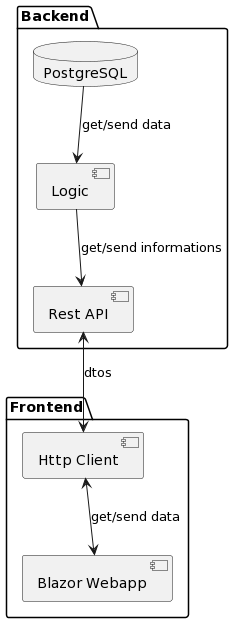
\includegraphics[scale=0.5]{pics/KomponentenDiagramm.png}
    \caption{Komponenten -- UML Diagramm}
    \label{fig:impl:KomponentenDiagramm}
\end{figure}

\newpage
Damit der Aufbau der .NET-Solution noch klarer wird ist nun die YAML-Datei dargestellt:

\lstinputlisting[style=yaml]{input-files/docker-compose.yml}

\newpage

Die verwendeten Entitäten und ihre Relationen im Backend sind in der folgenden Abbildung dargestellt.

\begin{figure}[H]
    \centering
    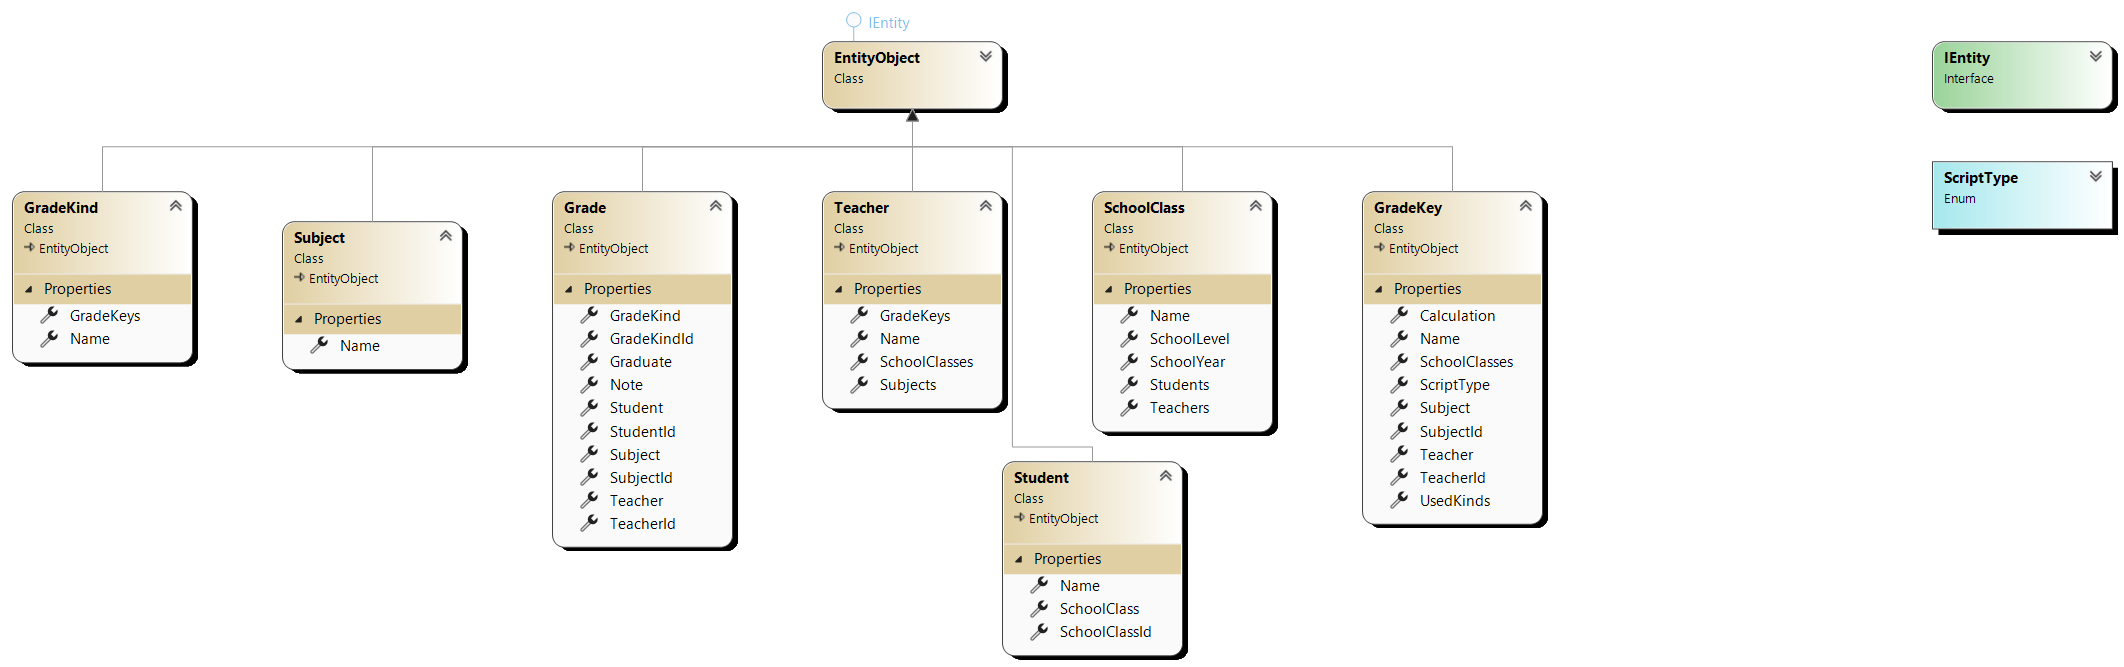
\includegraphics[scale=0.5]{pics/EntitiesClassDiagram.png}
    \caption{Entitäten -- UML Diagramm}
    \label{fig:impl:Entities}
\end{figure}

\newpage
Es gibt viele Möglichkeiten Skripte in eine Anwendung zu importieren.
Eine Möglichkeit ist die Skripte als Datei zu importieren.
Anstatt alle benötigten Daten direkt in den Code einzubetten oder sie manuell über die Befehlszeile einzugeben, 
können Entwickler eine oder mehrere Dateien als Input verwenden, die das Skript dann liest und verarbeitet.

\begin{figure}[H]
    \centering
    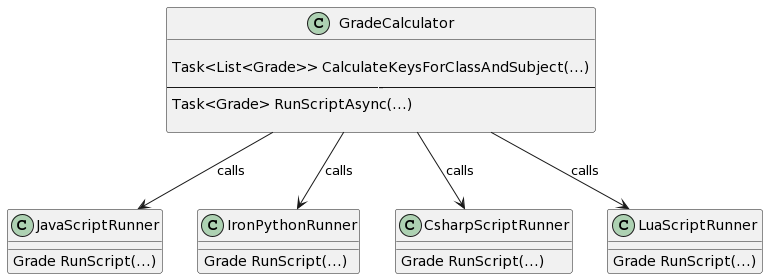
\includegraphics[scale=0.5]{pics/LogicClassDiagram.png}
    \caption{Logic Overview}
    \label{fig:impl:Logic}
\end{figure}


\newpage
Im folgenden Abschnitt  werden einige Code-Ausschnitte betrachtet, die zeigen, wie man solche Datei-Übergaben in den untersuchten Scriptsprachen realisieren kann. 

\begin{lstlisting}[language={[Sharp]C},caption=Code for Javascript,label=lst:impl:js]
    public class JavascriptRunner
    {
        public Grade RunScript(GradeKey key, List<Grade> grades)
        {
            var engine = new JintJsEngine();
            Grade result = new Grade();
            List<string>? logs = new List<string>();

            try
            {
                // Definiere eine Variable im JavaScript-Code, um die console.log-Ausgaben zu speichern
                engine.Execute("var consoleOutput = [];");

                // Definiere die console.log-Funktion im JavaScript-Code
                engine.Execute(@"
                                var console = {
                                    log: function() {
                                        consoleOutput.push(Array.from(arguments).join(' '));
                                    }
                                };
                            ");


                var gradeKindsList = JsonConvert.SerializeObject(key.UsedKinds);
                var gradesList = JsonConvert.SerializeObject(grades);

                engine.SetVariableValue("gradeKindsList", gradeKindsList);
                engine.SetVariableValue("gradesList", gradesList);

                if (key.Calculation != null)
                {
                    engine.Execute(key.Calculation);
                }

                //Die Ausgabe der console.log-Anweisungen als JSON-String
                string jsonOutput = engine.Evaluate<string>("JSON.stringify(consoleOutput)");

                // Konvertiere den JSON-String in eine Liste von strings
                if (jsonOutput != null)
                {
                    logs = JsonConvert.DeserializeObject<List<string>>(jsonOutput);

                    if (logs != null)
                    {
                        DisplayOutput(logs);   
                    }
                }

                // Get Return from Script
                var resultGrade = engine.GetVariableValue("result");

                result.Teacher = key.Teacher;
                result.Graduate = Convert.ToInt32(resultGrade);
            }
            catch (Exception)
            {
                result.Teacher = null;
                result.Graduate = 0;
            }
            return result;
        }

        private static void DisplayOutput(List<string> logs)
        {
            foreach (string output in logs)
            {
                Debug.WriteLine(output);
            }
        }
    }
\end{lstlisting}


\begin{lstlisting}[language={[Sharp]C},caption=Code for NLua,label=lst:impl:nlua]
    /// <summary>
    /// Runs lua-scripts
    /// </summary>
    public class LuaScriptRunner
    {
        private readonly Lua state;

        public LuaScriptRunner()
        {
            this.state = new Lua();
        }

        public Grade RunScript(GradeKey key, List<Grade> grades)
        {
            if (key.Calculation == string.Empty || key.UsedKinds == null || grades == null)
            {
                throw new NullReferenceException("Not enough information for Calculation");
            }

            var code = key.Calculation;

            var result = new Grade();
            try
            {
                state.DoString(code);
                state.LoadCLRPackage();
                state["grades"] = grades;
                state.DoString(@"graduate = calculate()");
                result.Teacher = key.Teacher;
                var gr = state["graduate"];
                if (gr != null) 
                {
                    result.Graduate = Convert.ToInt32(gr);
                }
            }
            catch (Exception)
            {
                throw;
            }

            return result;
        }
    }
\end{lstlisting}

\newpage

\begin{lstlisting}[language={[Sharp]C},caption=Code for CsharpScripting,label=lst:impl:csc]
    public class CsScriptRunner
    {
        public static Grade RunScript(GradeKey key, List<Grade> grades)
        {
            var result = new Grade();

            // StringWriter erstellen, um die Ausgabe des Skripts zu erfassen
            StringWriter sw = new StringWriter();

            // Console.Out umleiten
            TextWriter originalOut = Console.Out;
            Console.SetOut(sw);
            try
            {                
                dynamic script = CSScript.Evaluator
                    .ReferenceAssemblyOf(typeof(GradeKey))
                    .ReferenceAssemblyOf(typeof(Grade))
                    .CompileCode(key.Calculation)
                    .CreateObject("*");
                
                var res = script.Calculate(key, grades);
                result.Teacher = key.Teacher;              
                result.Graduate = Convert.ToInt32(res);

            }
            catch (Exception)
            {
                result.Teacher = null;
                result.Graduate = 0;
            }
            finally
            {
                // Output ausgeben
                Debug.WriteLine(sw);
            }

            return result;
        }
    }
\end{lstlisting}


